\chapter{序論}

\section{研究背景}
スマートタグとは貴重品などに取り付け, 紛失した際に捜索を補助するデバイスである. 
補助の方法はタグが音を鳴らす方法と付近のスマートフォンと無線通信する方法が一般的である. 
近年こうした製品が普及しており, なくしものの対策に需要があることを示唆している. 
しかし特性上タグの取り付けが困難な物もある. 
例えば入れ歯は口内で使用するために衛生や防水, 日常生活の邪魔になるなどの理由で取り付けが難しい. 

\section{関連研究}
タグを必要としないなくしもの対策として, 草野\index{くさの@草野}らが提案する家庭内での移動マニピュレータによるベイズ推定と自然言語処理を用いた物品捜索手法がある. \cite{kusano}
この手法ではまず捜索範囲をいくつかのエリアに区切る. 
そして各エリアごとに過去そのエリアを捜索し捜索対象を発見した回数$\alpha$, 発見できなかった回数$\beta$を用い, 
捜索対象の存在確率を$ \alpha / (\alpha + \beta)$と定義し, 存在確率が大きいエリアを捜索する. 
また存在確率が最大のエリアが複数ある場合は移動マニピュレータが位置するエリアからの距離, ならびに自然言語処理によるエリア内の家具と捜索対象の関連性も考慮する. 

\begin{figure}[H]
    \begin{center}
        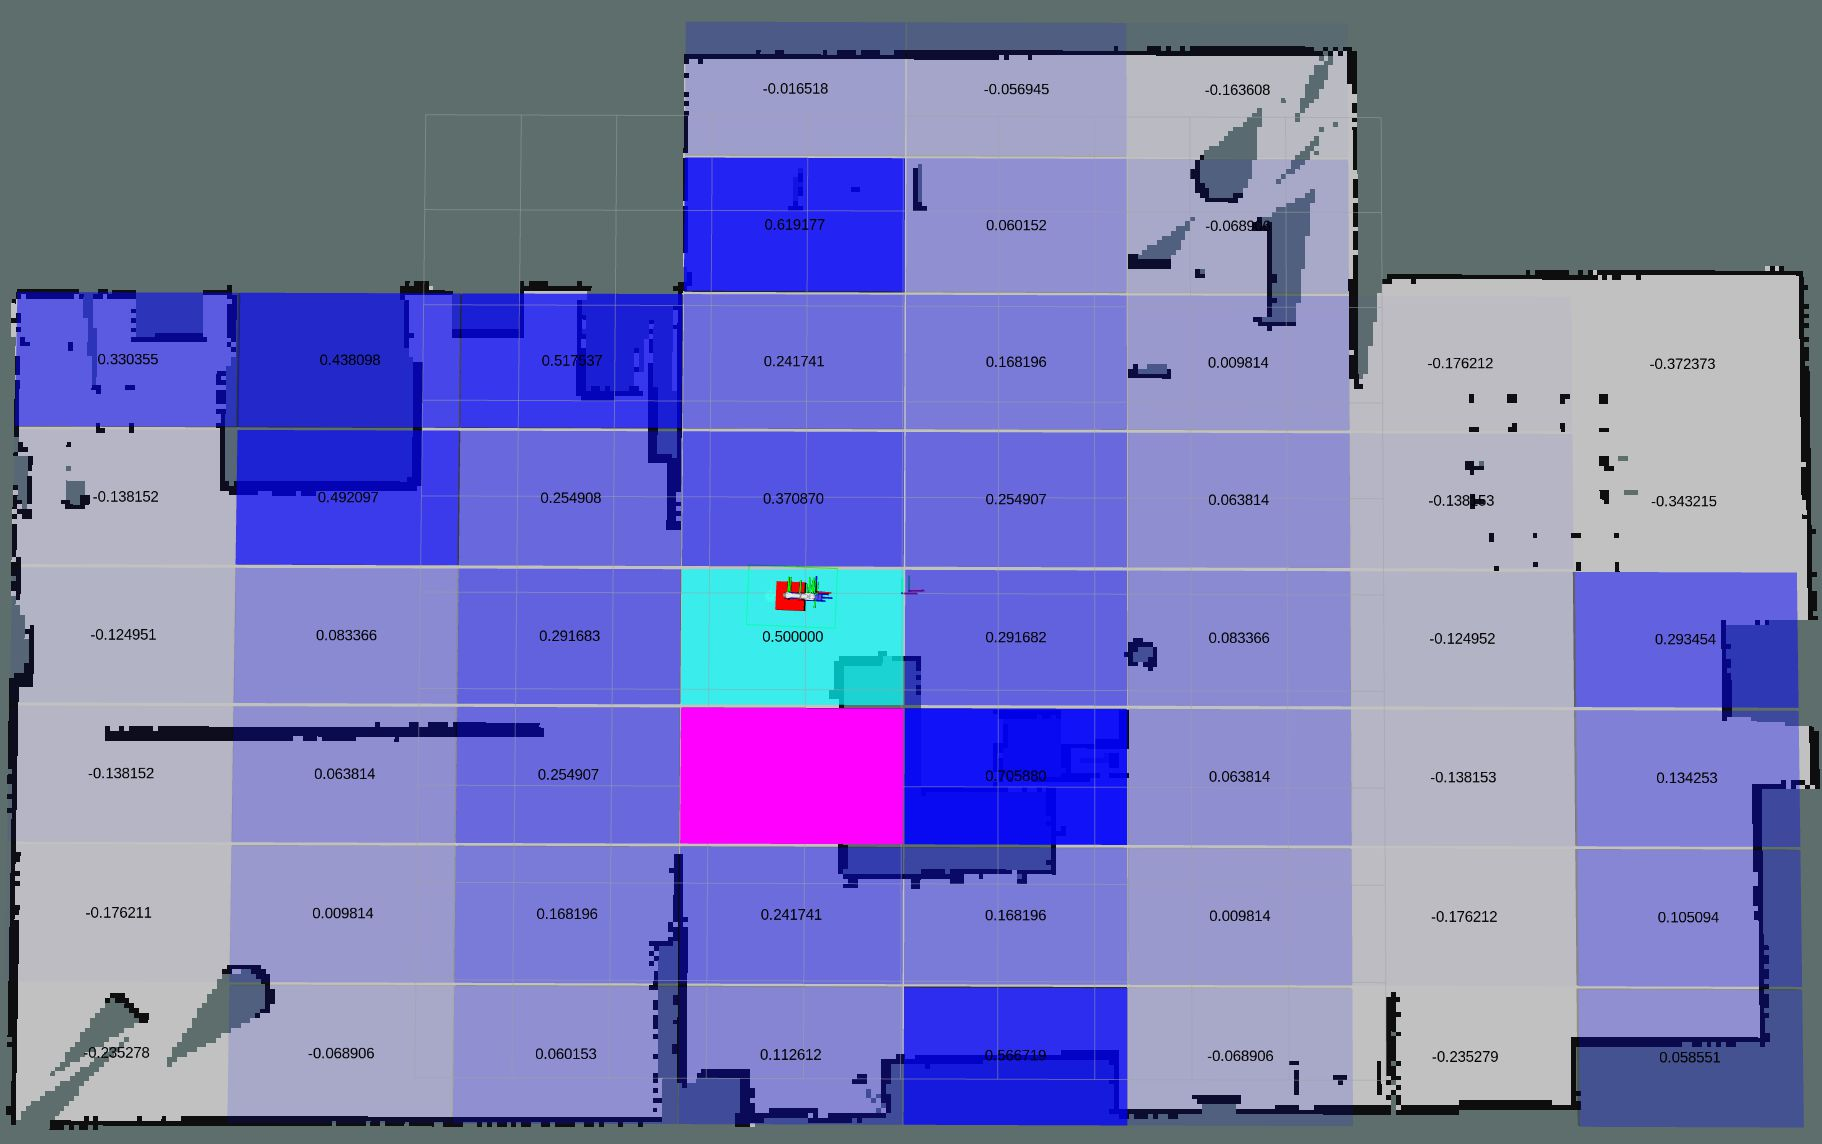
\includegraphics[width=0.8\linewidth]{figs/kusano.jpg}
        \caption{Existence probability of target object}
        \label{fig:kusano}
    \end{center}
\end{figure}

この手法は捜索する主体が移動マニピュレータであることと密接に結びついている. 
しかし現在, そうしたロボットはスマートタグの代替としては高価であり一般的な家庭での利用は難しい. 
% 移動マニピュレータの悪口は言いたくない
% 用途の広さ, 介護施設(=一般的の家庭でない環境)での利用等を考えれば高価とも言えないから

% *捜索範囲をいくつかのエリアに区切る
% *各エリアごとに過去そのエリアを捜索し捜索対象を発見した回数$\alpha$, 発見できなかった回数$\beta$を用いて, 捜索対象の存在確率を$\frac{\alpha}{\alpha + \beta}$と定義
% *存在確率が大きいエリアから捜索
% *存在確率が同じエリアがあった場合移動マニピュレータが位置するエリアからの距離, エリア内の家具と捜索対象との関連も考慮
% *移動マニピュレータであることと密接に結びついたアルゴリズム
% *移動マニピュレーターが要らないなくしもの対策がない

\section{研究目的}
なくしものは発生頻度が高くないため, 過去のなくしものから
利用者のなくしものが発生していない状況下での行動を反映することで最適化がより進む
確率論でモデル化
なくしものの位置の確率分布を計算
